% Capítulo I Marco Conceptual

% El marco conceptual o marco teórico, presenta de manera breve y concisa la teoría involucrada en el proyecto, es importante mantener un orden en la estructura del documento es indispensable manejar Capítulos, secciones y sub-secciones, estos comandos generan automáticamente el índice general que servirá a los asesores para navegar el documento. 

\chapter{ MARCO CONCEPTUAL }

\textit{El marco conceptual contiene de manera breve toda la teoría necesaria para poder entender el contenido de los siguientes capítulos.}

\section{ Ley de Ohm }

\begin{figure}[H]
	\begin{center}
 		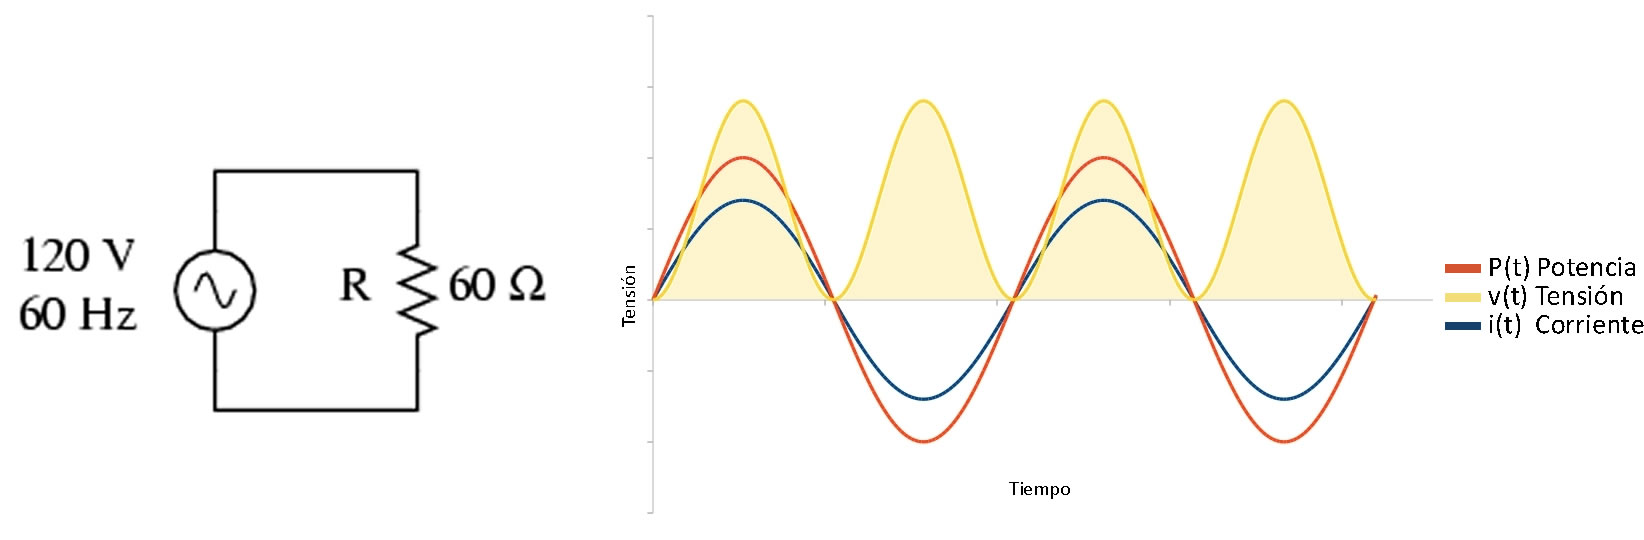
\includegraphics[width = .8\textwidth]{Tesis/Imagenes/resistiva.jpg}
 		\captionof{figure}{Comportamiento en el tiempo de una carga resistiva \cite{AC}} 
	\label{RESISTIVA}
    \end{center} 
\end{figure}

Es una de las leyes fundamentales de la electrodinámica, estrechamente vinculada a los valores de las unidades básicas presentes en cualquier circuito eléctrico como son:

\begin{equation}
V = IR  
\label{voltaje}
\end{equation}

A las formula de en la ecuación \ref{voltaje} se le conoce como la Ley de Ohm

\subsection{ Despeje de la ley de ohm }

Es posible despejar la corriente de la ecuación \ref{voltaje} para poder obtener la corriente total que fluye por el sistema dando como resultado la ecuación \ref{corriente} es decir:

\begin{equation}
I = V/R  
\label{corriente}
\end{equation}

\begin{itemize}
\item Tensión o voltaje $E$, en volt ($V$).
\item Intensidad de la corriente $I$, en ampere ($A$).
\item Resistencia $R$ en ohm ( $\Omega$ ) de la carga o consumidor conectado al circuito.
\end{itemize}

\section{ Resumen del capitulo 1 }

\textit{Para ayudar al lector se recomienda agregar una sección de resumen del capitulo, esto permite al lector resumir y entender que es los que leyó y dar un repaso del contenido del capitulo así como guiarlo con una referencia de entrada al capitulo siguiente.}


% FIN de Capítulo I Marco Conceptual

